\documentclass{standalone}
\usepackage{tikz}

\usetikzlibrary{matrix,positioning,shapes.arrows,fit}

\tikzset{ 
table/.style={
  matrix of nodes,
  row sep=-\pgflinewidth,
  column sep=-\pgflinewidth,
  nodes={
    rectangle,draw,
    text width=0.5cm,
    %minimum width=0.75cm,
    %minimum height=0.75cm,
    align=center},
  text depth=0.125cm,
  text height=0.25cm,
  nodes in empty cells,
  outer sep=0cm,
  },
%texto/.style={font=\footnotesize\sffamily},
%title/.style={font=\small\sffamily}
}

\begin{document}
    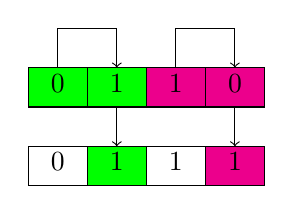
\begin{tikzpicture}[
        every node/.style = {
            %draw, rectangle, 
            minimum width=0.75cm,
            minimum height=0.5cm,
            outer sep=0cm, inner sep=0cm,
            node distance=0cm
        }
    ]
    \matrix [table] (s0)
    {
        \node[fill=green] (s0-1-1) {0}; & 
        \node[fill=green] (s0-1-2) {1}; & 
        \node[fill=magenta] (s0-1-3) {1}; & 
        \node[fill=magenta] (s0-1-4) {0}; \\
    };
    \matrix [table, below of=s0, node distance=1cm] (s1)
    {
        0 & \node[fill=green] (s1-1-2) {1}; & 
        1 & \node[fill=magenta] (s1-1-4) {1}; \\
    };
    \draw[->] (s0-1-1.north) -- ++(0,0.5) -| (s0-1-2.north);
    \draw[->] (s0-1-3.north) -- ++(0,0.5) -| (s0-1-4.north);
    \draw[->] (s0-1-2.south) -- (s1-1-2.north);
    \draw[->] (s0-1-4.south) -- (s1-1-4.north);
    \end{tikzpicture}
\end{document}